%----------------------------------------------------------------------------------------
%	INTRODUCTION
%----------------------------------------------------------------------------------------
\section{Introduction}

TODO: Introduction to the project and motivation behind it.

\subsection{The project}

TODO: Rough summary of the idea of the project.
How did the idea come up?
What is the project about?

\subsection{Background on computer vision based classification tasks}

TODO: Short introduction into the fields of machine learning, computer vision, and to artificial neural networks. Prospects and challenges of both on a general basis with respect to our issue. This part is kept brief.

\subsection{Background on sorting asparagus}

\begin{figure}[h]
	\centering
	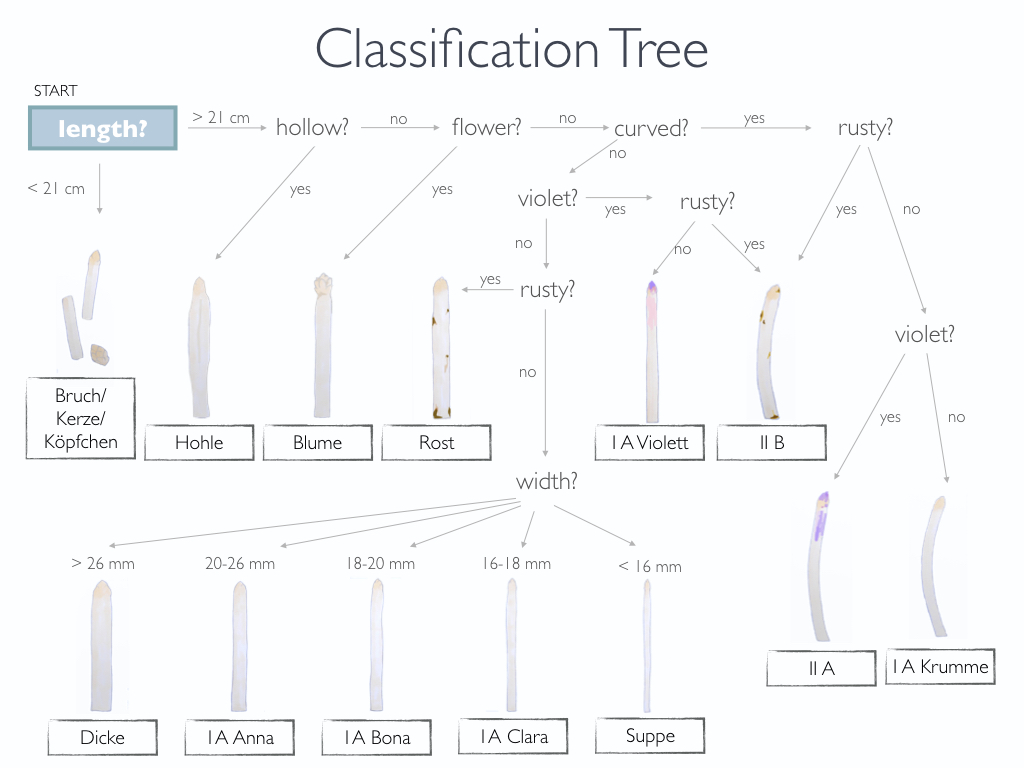
\includegraphics[scale=0.35]{Figures/chapter01/fig_tree_with_title}
	\decoRule
	\caption[Decision tree for labels]{The decision tree for attributing a label to the asparagus as to the sorting rules of the asparagus farm "Gut Holsterfeld". Starting from the upper left corner of the image binary decisions are made until a label is reached (except for Width).}
	\label{fig:LabelTree}
\end{figure}

TODO: What is the main focus during the sorting process, i.e. why do you need to sort asparagus and in which classes do you sort it? \\
What problems and challenges will be met - including the difference of challenge for humans vs. machines. \\
Including the description of the labels as sorted by Hof Gut Holsterfeld (Figure~\ref{fig:LabelTree}).


\subsection{Expected outcome vs. actual outcome of the project}

Based on the literature review, we aimed to improve the current sorting performance of the XX machine at the local asparagus farm “Spargelhof Gut Holsterfeld”. In this report, we investigated techniques from computer vision, both classical and deep learning based approaches. We expected to reach a result which is able to classify asparagus images into 13 different classes better than the current standard. For the initial performance of the sorting machine, no reliable accuracy of correctly sorted asparagus pieces is available, but between three and six workers are employed to re-sort wrongly classified asparagus pieces. The farmer himself assumes an accuracy of not more than 70\%. \\
 
An advantage of our project is that it was directly supported by the local asparagus farm, providing training data and allowing us to evaluate our proposed solutions in a real environment during the asparagus harvesting season 2020. \\
\\
However, there was a misunderstanding between us and the supporting asparagus farm about the kind of data we need. The existing images were too few, and also unlabelled. Therefore, we spent the first two and a half months with data acquisition instead of starting with preprocessing as we originally planned. Throughout the harvesting season 2019, we continuously went to the asparagus farm and collected unlabelled asparagus images during the normal harvesting procedure. For a small amount of asparagus pieces (xx in total), we collected labelled data by taking images of pre-sorted asparagus pieces. Pre-sorted in this context means that the asparagus pieces were sorted by the sorting machine and if needed re-sorted manually by professional workers. \\
The number of labelled images is insufficient to learn classes using deep learning approaches~\citep{russakovsky2013detecting} ~\citep{russakovsky2010attribute} (\url{https://petewarden.com/2017/12/14/how-many-images-do-you-need-to-train-a-neural-network/}). Therefore, we spent six months preprocessing and labelling the data manually. Preprocessing involved: organizing the large number of images, renaming the files, so that the three images of one asparagus piece can be accessed together, and performing automatic feature extractions (ref to preprocessing).To label the images by hand, we wrote a custom application (reference hand-label-assistant). The final labelled data set contains over 10.000 (genaue Zahl an stangen) labelled asparagus pieces. Next, we worked on numerous classical and deep learning approaches (ref to chap 4). We reached several very interesting results which will be discussed in Chapter 4. Although we developed an end-to-end prototype, we did not deploy it onto the sorting machine for the harvesting season 2020. Even though some of our results are highly promising, it is therefore difficult to compare it to the current performance of the machine. \\
 \\
Hier noch ein Absatz mit den Inhalten aus der Conclusion – sobald diese steht. 



